\documentclass[11pt,]{article}
\usepackage[left=1in,top=1in,right=1in,bottom=1in]{geometry}
\newcommand*{\authorfont}{\fontfamily{phv}\selectfont}
\usepackage[]{mathpazo}


  \usepackage[T1]{fontenc}
  \usepackage[utf8]{inputenc}




\usepackage{abstract}
\renewcommand{\abstractname}{}    % clear the title
\renewcommand{\absnamepos}{empty} % originally center

\renewenvironment{abstract}
 {{%
    \setlength{\leftmargin}{0mm}
    \setlength{\rightmargin}{\leftmargin}%
  }%
  \relax}
 {\endlist}

\makeatletter
\def\@maketitle{%
  \newpage
%  \null
%  \vskip 2em%
%  \begin{center}%
  \let \footnote \thanks
    {\fontsize{18}{20}\selectfont\raggedright  \setlength{\parindent}{0pt} \@title \par}%
}
%\fi
\makeatother




\setcounter{secnumdepth}{0}

\usepackage{color}
\usepackage{fancyvrb}
\newcommand{\VerbBar}{|}
\newcommand{\VERB}{\Verb[commandchars=\\\{\}]}
\DefineVerbatimEnvironment{Highlighting}{Verbatim}{commandchars=\\\{\}}
% Add ',fontsize=\small' for more characters per line
\usepackage{framed}
\definecolor{shadecolor}{RGB}{248,248,248}
\newenvironment{Shaded}{\begin{snugshade}}{\end{snugshade}}
\newcommand{\AlertTok}[1]{\textcolor[rgb]{0.94,0.16,0.16}{#1}}
\newcommand{\AnnotationTok}[1]{\textcolor[rgb]{0.56,0.35,0.01}{\textbf{\textit{#1}}}}
\newcommand{\AttributeTok}[1]{\textcolor[rgb]{0.77,0.63,0.00}{#1}}
\newcommand{\BaseNTok}[1]{\textcolor[rgb]{0.00,0.00,0.81}{#1}}
\newcommand{\BuiltInTok}[1]{#1}
\newcommand{\CharTok}[1]{\textcolor[rgb]{0.31,0.60,0.02}{#1}}
\newcommand{\CommentTok}[1]{\textcolor[rgb]{0.56,0.35,0.01}{\textit{#1}}}
\newcommand{\CommentVarTok}[1]{\textcolor[rgb]{0.56,0.35,0.01}{\textbf{\textit{#1}}}}
\newcommand{\ConstantTok}[1]{\textcolor[rgb]{0.00,0.00,0.00}{#1}}
\newcommand{\ControlFlowTok}[1]{\textcolor[rgb]{0.13,0.29,0.53}{\textbf{#1}}}
\newcommand{\DataTypeTok}[1]{\textcolor[rgb]{0.13,0.29,0.53}{#1}}
\newcommand{\DecValTok}[1]{\textcolor[rgb]{0.00,0.00,0.81}{#1}}
\newcommand{\DocumentationTok}[1]{\textcolor[rgb]{0.56,0.35,0.01}{\textbf{\textit{#1}}}}
\newcommand{\ErrorTok}[1]{\textcolor[rgb]{0.64,0.00,0.00}{\textbf{#1}}}
\newcommand{\ExtensionTok}[1]{#1}
\newcommand{\FloatTok}[1]{\textcolor[rgb]{0.00,0.00,0.81}{#1}}
\newcommand{\FunctionTok}[1]{\textcolor[rgb]{0.00,0.00,0.00}{#1}}
\newcommand{\ImportTok}[1]{#1}
\newcommand{\InformationTok}[1]{\textcolor[rgb]{0.56,0.35,0.01}{\textbf{\textit{#1}}}}
\newcommand{\KeywordTok}[1]{\textcolor[rgb]{0.13,0.29,0.53}{\textbf{#1}}}
\newcommand{\NormalTok}[1]{#1}
\newcommand{\OperatorTok}[1]{\textcolor[rgb]{0.81,0.36,0.00}{\textbf{#1}}}
\newcommand{\OtherTok}[1]{\textcolor[rgb]{0.56,0.35,0.01}{#1}}
\newcommand{\PreprocessorTok}[1]{\textcolor[rgb]{0.56,0.35,0.01}{\textit{#1}}}
\newcommand{\RegionMarkerTok}[1]{#1}
\newcommand{\SpecialCharTok}[1]{\textcolor[rgb]{0.00,0.00,0.00}{#1}}
\newcommand{\SpecialStringTok}[1]{\textcolor[rgb]{0.31,0.60,0.02}{#1}}
\newcommand{\StringTok}[1]{\textcolor[rgb]{0.31,0.60,0.02}{#1}}
\newcommand{\VariableTok}[1]{\textcolor[rgb]{0.00,0.00,0.00}{#1}}
\newcommand{\VerbatimStringTok}[1]{\textcolor[rgb]{0.31,0.60,0.02}{#1}}
\newcommand{\WarningTok}[1]{\textcolor[rgb]{0.56,0.35,0.01}{\textbf{\textit{#1}}}}
\usepackage{longtable,booktabs}

\usepackage{graphicx,grffile}
\makeatletter
\def\maxwidth{\ifdim\Gin@nat@width>\linewidth\linewidth\else\Gin@nat@width\fi}
\def\maxheight{\ifdim\Gin@nat@height>\textheight\textheight\else\Gin@nat@height\fi}
\makeatother
% Scale images if necessary, so that they will not overflow the page
% margins by default, and it is still possible to overwrite the defaults
% using explicit options in \includegraphics[width, height, ...]{}
\setkeys{Gin}{width=\maxwidth,height=\maxheight,keepaspectratio}


\title{Predicting Admission Probability in U.S Grad school using Linear Models
and Machine Learning Algorithms \thanks{S.V Miller for providing the Pandoc template: github.com/svmiller}  }



\author{\Large Arumugam Thiagarajan\vspace{0.05in} \newline\normalsize\emph{Professional Certificate in Data Science, Harvard University}  }


\date{}

\usepackage{titlesec}

\titleformat*{\section}{\normalsize\bfseries}
\titleformat*{\subsection}{\normalsize\itshape}
\titleformat*{\subsubsection}{\normalsize\itshape}
\titleformat*{\paragraph}{\normalsize\itshape}
\titleformat*{\subparagraph}{\normalsize\itshape}





\newtheorem{hypothesis}{Hypothesis}
\usepackage{setspace}


% set default figure placement to htbp
\makeatletter
\def\fps@figure{htbp}
\makeatother

\usepackage{booktabs}
\usepackage{longtable}
\usepackage{array}
\usepackage{multirow}
\usepackage{wrapfig}
\usepackage{float}
\usepackage{colortbl}
\usepackage{pdflscape}
\usepackage{tabu}
\usepackage{threeparttable}
\usepackage{threeparttablex}
\usepackage[normalem]{ulem}
\usepackage{makecell}
\usepackage{xcolor}

% move the hyperref stuff down here, after header-includes, to allow for - \usepackage{hyperref}

\makeatletter
\@ifpackageloaded{hyperref}{}{%
\ifxetex
  \PassOptionsToPackage{hyphens}{url}\usepackage[setpagesize=false, % page size defined by xetex
              unicode=false, % unicode breaks when used with xetex
              xetex]{hyperref}
\else
  \PassOptionsToPackage{hyphens}{url}\usepackage[draft,unicode=true]{hyperref}
\fi
}

\@ifpackageloaded{color}{
    \PassOptionsToPackage{usenames,dvipsnames}{color}
}{%
    \usepackage[usenames,dvipsnames]{color}
}
\makeatother
\hypersetup{breaklinks=true,
            bookmarks=true,
            pdfauthor={Arumugam Thiagarajan (Professional Certificate in Data Science, Harvard University)},
             pdfkeywords = {house rent, machine learning, linear models},  
            pdftitle={Predicting Admission Probability in U.S Grad school using Linear Models
and Machine Learning Algorithms},
            colorlinks=true,
            citecolor=blue,
            urlcolor=blue,
            linkcolor=magenta,
            pdfborder={0 0 0}}
\urlstyle{same}  % don't use monospace font for urls

% Add an option for endnotes. -----


% add tightlist ----------
\providecommand{\tightlist}{%
\setlength{\itemsep}{0pt}\setlength{\parskip}{0pt}}

% add some other packages ----------

% \usepackage{multicol}
% This should regulate where figures float
% See: https://tex.stackexchange.com/questions/2275/keeping-tables-figures-close-to-where-they-are-mentioned
\usepackage[section]{placeins}


\begin{document}
	
% \pagenumbering{arabic}% resets `page` counter to 1 
%
% \maketitle

{% \usefont{T1}{pnc}{m}{n}
\setlength{\parindent}{0pt}
\thispagestyle{plain}
{\fontsize{18}{20}\selectfont\raggedright 
\maketitle  % title \par  

}

{
   \vskip 13.5pt\relax \normalsize\fontsize{11}{12} 
\textbf{\authorfont Arumugam Thiagarajan} \hskip 15pt \emph{\small Professional Certificate in Data Science, Harvard University}   

}

}








\begin{abstract}

    \hbox{\vrule height .2pt width 39.14pc}

    \vskip 8.5pt % \small 

\noindent The project develops and compares a linear and a suite of machine
learning algorithms that predicts the admission probabilty of applicants
to United States Graduate Schools. The applicant characterisitics and
academic standings such as, TOEFL scores, GRE scores, Cumulative Grade
Point Average (CGPA), Letter of Recommendation (LOR) and Statement of
Purpose are some of the attributes that are used to predict their
admission probability to universities. A regression based approach was
used and the dataset was explored for trends, cleansed with relevant
attributes and models were built using linear regression and machine
learning algorithm. Training and validation datasets were estbalished at
a 50:50 proportion at random. Root Mean Square and R2 values were used
as measures of performance and the results revealed that linear
regression model and an ensemble of machine learning models both
predicted the outcomes with the same level of accuracy. The RMSE values
were at 0.066 with an r2 value of 0.88


\vskip 8.5pt \noindent \emph{Keywords}: house rent, machine learning, linear models \par

    \hbox{\vrule height .2pt width 39.14pc}



\end{abstract}


\vskip -8.5pt

{
\hypersetup{linkcolor=black}
\setcounter{tocdepth}{2}
\tableofcontents
}

 % removetitleabstract

\noindent  

\hypertarget{executive-summary}{%
\section{Executive Summary}\label{executive-summary}}

This project builds a mathematical model that predicts the house rents
in selected Brazilian cities.

\hypertarget{objective}{%
\section{Objective}\label{objective}}

Predict the admission rates in United States Grad School using the
academic scores of the applicants, and the university rankings. Both
general linear models and machine learning algorithms will be used and
their performances will be compared. Root Mean Squarewill be used as the
measure of performance for the model.

\#Install and load up the libraries that are required for the analysis
to run.

\hypertarget{load-the-data-that-is-used-for-the-development-of-the-model.}{%
\section{Load the data that is used for the development of the
model.}\label{load-the-data-that-is-used-for-the-development-of-the-model.}}

The original data is available for public in the following url:
\url{https://www.kaggle.com/}

Since a direct download from kaggle requires an authentication, the
whole dataset is uploaded to github account. The data and codes can be
downloaded from the following github repository.
\url{https://github.com/HexyCodes/}

This dataset contains, 400 rows of data and 8 attributes.

\#Data characteristics and Summary

\begin{Shaded}
\begin{Highlighting}[]
\NormalTok{adm=}\KeywordTok{read.csv}\NormalTok{(}\StringTok{"~/Documents/Harvard/R/CapStone/Admission/US_grad_admission.csv"}\NormalTok{, }
             \DataTypeTok{stringsAsFactors =}\NormalTok{ F)}
\KeywordTok{dim}\NormalTok{(adm) }\CommentTok{# find the dimensions of the data.frame}
\end{Highlighting}
\end{Shaded}

\begin{verbatim}
## [1] 400   9
\end{verbatim}

\hypertarget{exploratory-data-analysis}{%
\section{Exploratory Data Analysis}\label{exploratory-data-analysis}}

Here the data is analyzed for their summarized characteristics through
visualization. This step allows us to find the patterns, trends and any
anamolies if exist in the data. The serial number column has been
removed to cleanse the data removing unrelated column. This was an
obvious choice as this will add unncessary noise to the modeling
process.

\begin{Shaded}
\begin{Highlighting}[]
\KeywordTok{class}\NormalTok{(adm)}
\end{Highlighting}
\end{Shaded}

\begin{verbatim}
## [1] "data.frame"
\end{verbatim}

\begin{Shaded}
\begin{Highlighting}[]
\KeywordTok{head}\NormalTok{(adm,}\DecValTok{5}\NormalTok{) }\CommentTok{# look at the data type of columns}
\end{Highlighting}
\end{Shaded}

\begin{verbatim}
##   Serial.No. GRE.Score TOEFL.Score University.Rating SOP LOR CGPA Research
## 1          1       337         118                 4 4.5 4.5 9.65        1
## 2          2       324         107                 4 4.0 4.5 8.87        1
## 3          3       316         104                 3 3.0 3.5 8.00        1
## 4          4       322         110                 3 3.5 2.5 8.67        1
## 5          5       314         103                 2 2.0 3.0 8.21        0
##   Chance.of.Admit
## 1            0.92
## 2            0.76
## 3            0.72
## 4            0.80
## 5            0.65
\end{verbatim}

\begin{Shaded}
\begin{Highlighting}[]
\KeywordTok{print}\NormalTok{(}\KeywordTok{anyNA}\NormalTok{(adm))}\CommentTok{# check for missing values}
\end{Highlighting}
\end{Shaded}

\begin{verbatim}
## [1] FALSE
\end{verbatim}

\begin{Shaded}
\begin{Highlighting}[]
\KeywordTok{summary}\NormalTok{(adm) }\CommentTok{# quantile distribution of the predicted values}
\end{Highlighting}
\end{Shaded}

\begin{verbatim}
##    Serial.No.      GRE.Score      TOEFL.Score    University.Rating
##  Min.   :  1.0   Min.   :290.0   Min.   : 92.0   Min.   :1.000    
##  1st Qu.:100.8   1st Qu.:308.0   1st Qu.:103.0   1st Qu.:2.000    
##  Median :200.5   Median :317.0   Median :107.0   Median :3.000    
##  Mean   :200.5   Mean   :316.8   Mean   :107.4   Mean   :3.087    
##  3rd Qu.:300.2   3rd Qu.:325.0   3rd Qu.:112.0   3rd Qu.:4.000    
##  Max.   :400.0   Max.   :340.0   Max.   :120.0   Max.   :5.000    
##       SOP           LOR             CGPA          Research     
##  Min.   :1.0   Min.   :1.000   Min.   :6.800   Min.   :0.0000  
##  1st Qu.:2.5   1st Qu.:3.000   1st Qu.:8.170   1st Qu.:0.0000  
##  Median :3.5   Median :3.500   Median :8.610   Median :1.0000  
##  Mean   :3.4   Mean   :3.453   Mean   :8.599   Mean   :0.5475  
##  3rd Qu.:4.0   3rd Qu.:4.000   3rd Qu.:9.062   3rd Qu.:1.0000  
##  Max.   :5.0   Max.   :5.000   Max.   :9.920   Max.   :1.0000  
##  Chance.of.Admit 
##  Min.   :0.3400  
##  1st Qu.:0.6400  
##  Median :0.7300  
##  Mean   :0.7244  
##  3rd Qu.:0.8300  
##  Max.   :0.9700
\end{verbatim}

\begin{Shaded}
\begin{Highlighting}[]
\NormalTok{adm}\OperatorTok\KeywordTok{ggplot}\NormalTok{(}\KeywordTok{aes}\NormalTok{(}\DataTypeTok{x=}\NormalTok{Chance.of.Admit))}\OperatorTok{+}\KeywordTok{geom_density}\NormalTok{(}\DataTypeTok{bins =} \DecValTok{20}\NormalTok{, }\DataTypeTok{fill=}\StringTok{"blue"}\NormalTok{) }\OperatorTok{+}\StringTok{ }\KeywordTok{theme_bw}\NormalTok{() }
\end{Highlighting}
\end{Shaded}

\begin{verbatim}
## Warning: Ignoring unknown parameters: bins
\end{verbatim}

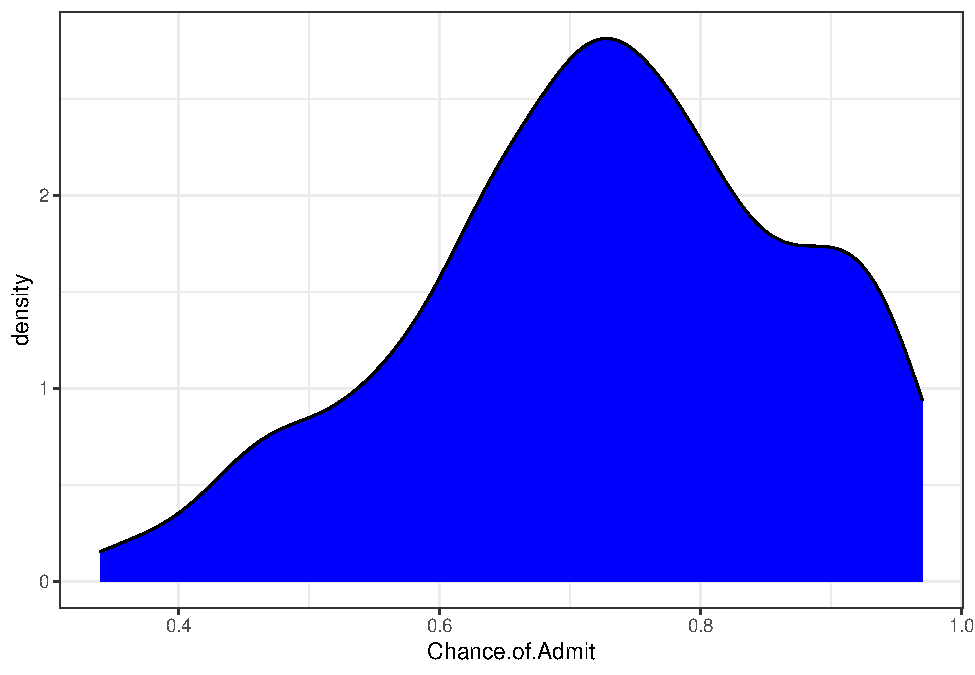
\includegraphics{USGradAdmission_files/figure-latex/unnamed-chunk-3-1.pdf}

\begin{Shaded}
\begin{Highlighting}[]
  \CommentTok{# distribution }
\CommentTok{#pattern of the predicted value}
\KeywordTok{qqnorm}\NormalTok{(adm}\OperatorTok{$}\NormalTok{Chance.of.Admit)}
\end{Highlighting}
\end{Shaded}

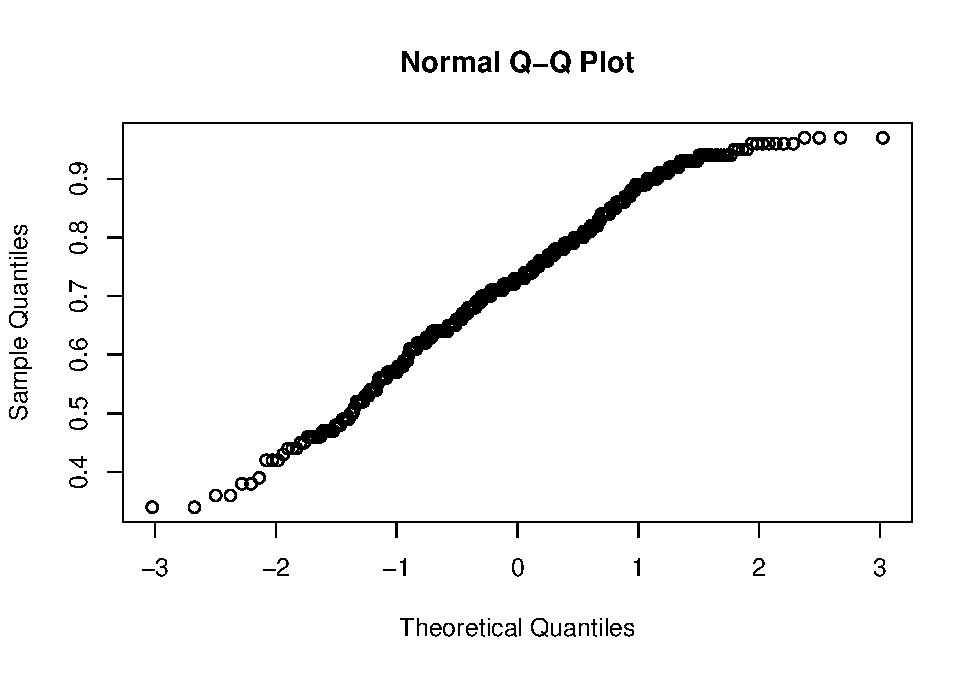
\includegraphics{USGradAdmission_files/figure-latex/unnamed-chunk-3-2.pdf}

\begin{Shaded}
\begin{Highlighting}[]
\NormalTok{adm}\OperatorTok\NormalTok{dplyr}\OperatorTok{::}\KeywordTok{select}\NormalTok{(}\OperatorTok{-}\NormalTok{Serial.No.)->adm }\CommentTok{# Remove Serial number from the daa. }
\KeywordTok{plot_density}\NormalTok{(adm, }
             \DataTypeTok{geom_density_args =} \KeywordTok{list}\NormalTok{(}\StringTok{"fill"}\NormalTok{=}\StringTok{"blue"}\NormalTok{, }
                                      \StringTok{"alpha"}\NormalTok{=}\FloatTok{0.6}\NormalTok{)) }\CommentTok{# distribution all predictors in the data frame}
\end{Highlighting}
\end{Shaded}

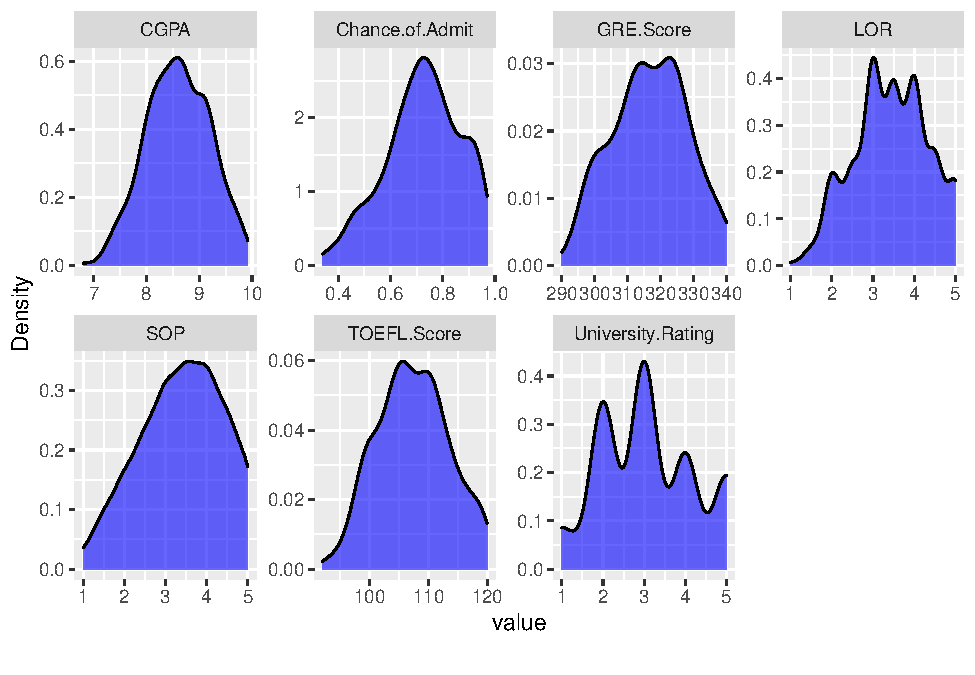
\includegraphics{USGradAdmission_files/figure-latex/unnamed-chunk-3-3.pdf}

\hypertarget{removing-extreme-values}{%
\section{Removing Extreme values}\label{removing-extreme-values}}

Histogram and boxplots of the admission vector indicates a normal
distribution for all the features. It is a recommended practice to
examine the dataset for outliers. Therefore, a Inter quantile range
(IQR) methodology was used to identify the ``proposed outliers''. First,
the Q1 and Q3 quantile are identified, then the IRQ was calculated as
teh difference between the Q3 and Q1. The range of values that exist
below the IQR\emph{1.5 or above IQR}1.5 were eliminated for this
project. From the results only two rows were identified as potential
outliers. Considering the low occurrence of these values, the dataset is
being used as such with no removal of outliers.

\begin{Shaded}
\begin{Highlighting}[]
\KeywordTok{any}\NormalTok{(}\KeywordTok{is.na}\NormalTok{(adm)) }\CommentTok{# Checking for any missing values}
\end{Highlighting}
\end{Shaded}

\begin{verbatim}
## [1] FALSE
\end{verbatim}

\begin{Shaded}
\begin{Highlighting}[]
\NormalTok{IQR.outliers <-}\StringTok{ }\ControlFlowTok{function}\NormalTok{(x) \{}
  \ControlFlowTok{if}\NormalTok{(}\KeywordTok{any}\NormalTok{(}\KeywordTok{is.na}\NormalTok{(x)))}
    \KeywordTok{stop}\NormalTok{(}\StringTok{"x is missing values"}\NormalTok{)}
  \ControlFlowTok{if}\NormalTok{(}\OperatorTok{!}\KeywordTok{is.numeric}\NormalTok{(x))}
    \KeywordTok{stop}\NormalTok{(}\StringTok{"x is not numeric"}\NormalTok{)}
\NormalTok{  Q3<-}\KeywordTok{quantile}\NormalTok{(x,}\FloatTok{0.75}\NormalTok{)}
\NormalTok{  Q1<-}\KeywordTok{quantile}\NormalTok{(x,}\FloatTok{0.25}\NormalTok{)}
\NormalTok{  IQR<-(Q3}\OperatorTok{-}\NormalTok{Q1)}
\NormalTok{  left<-}\StringTok{ }\NormalTok{(Q1}\OperatorTok{-}\NormalTok{(}\FloatTok{1.5}\OperatorTok{*}\NormalTok{IQR))}
  \KeywordTok{print}\NormalTok{(left)}

\NormalTok{  right<-}\StringTok{ }\NormalTok{(Q3}\OperatorTok{+}\NormalTok{(}\FloatTok{1.5}\OperatorTok{*}\NormalTok{IQR))}
    \KeywordTok{print}\NormalTok{(right)}
  \KeywordTok{c}\NormalTok{(x[x }\OperatorTok{<}\NormalTok{left],x[x}\OperatorTok{>}\NormalTok{right])}
\NormalTok{\}}



\NormalTok{outliers=}\KeywordTok{IQR.outliers}\NormalTok{(adm}\OperatorTok{$}\NormalTok{Chance.of.Admit)}
\end{Highlighting}
\end{Shaded}

\begin{verbatim}
##   25% 
## 0.355 
##   75% 
## 1.115
\end{verbatim}

\hypertarget{data-exploration}{%
\section{Data Exploration}\label{data-exploration}}

\hypertarget{check-for-correlations}{%
\subsection{Check for correlations}\label{check-for-correlations}}

The dataset is examined for correlations among the different attributes.
There seems to a be strong correlations (\textgreater{}50\%) between all
of the features, such as GRE. Score, TOEFL. Score, University. Rating,
SOP, LOR, CGPA and Research. The boxplot on the important feature reveal
a linear relationship with these features. This is an interesting trend,
because many of these characteristics have confounding effects or
colinearity that exist with them. For instance, a person scoring high in
GRE has high probability of scoring high in TOEFL and potentially wrote
a worthy statemnent of purpose. Therefore, it is essential to examinte
partial correlation coefficients of these attributes on the admisssion
chances.

\begin{Shaded}
\begin{Highlighting}[]
\CommentTok{# Converting the data into matrix format for conduction correlation analysis}
\KeywordTok{data.matrix}\NormalTok{(adm)->adm_mat }
\CommentTok{# plotting the hrent matrix results}
\KeywordTok{plot_correlation}\NormalTok{(adm_mat) }
\end{Highlighting}
\end{Shaded}

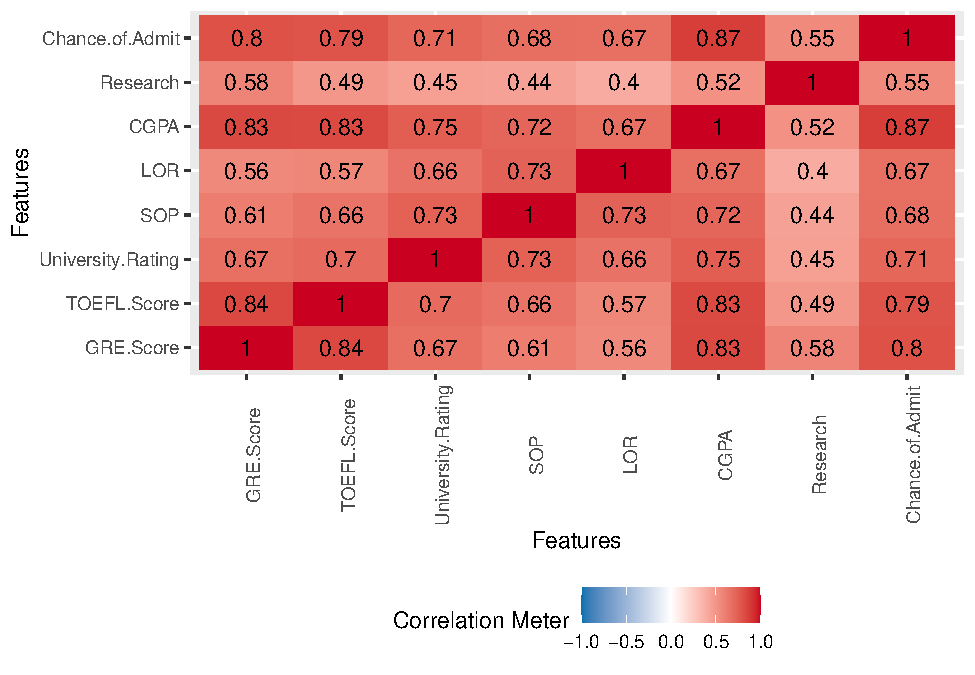
\includegraphics{USGradAdmission_files/figure-latex/unnamed-chunk-5-1.pdf}

\begin{Shaded}
\begin{Highlighting}[]
\CommentTok{# plotting the correlation strength through size of squares.}
\KeywordTok{corrplot}\NormalTok{(}\KeywordTok{cor}\NormalTok{(adm_mat), }\DataTypeTok{method =} \StringTok{"square"}\NormalTok{) }
\end{Highlighting}
\end{Shaded}

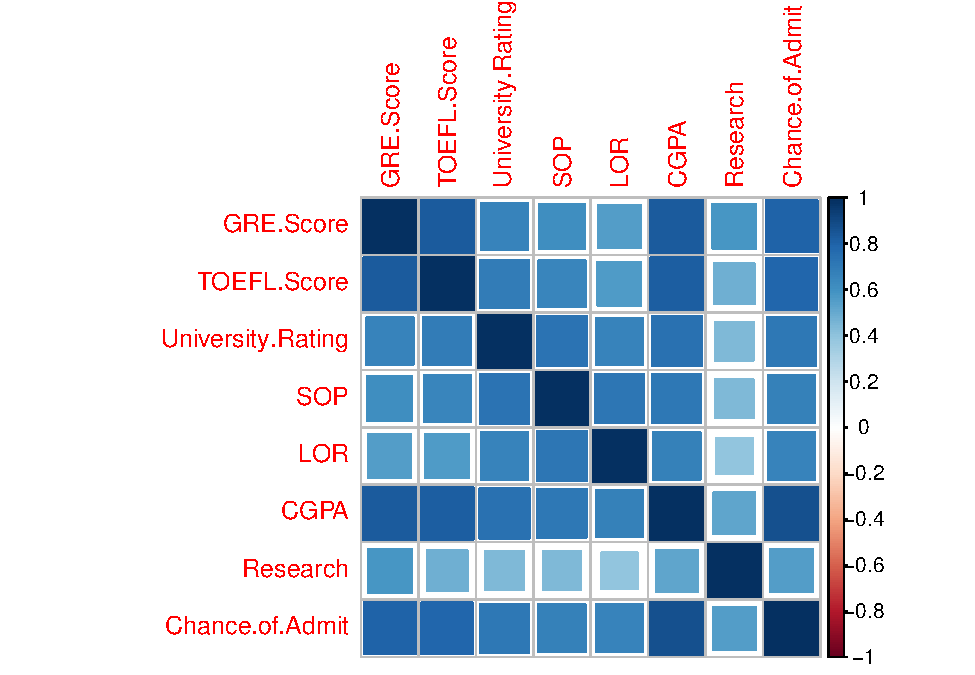
\includegraphics{USGradAdmission_files/figure-latex/unnamed-chunk-5-2.pdf}

\hypertarget{visualizing-the-relationship}{%
\subsection{Visualizing the
relationship}\label{visualizing-the-relationship}}

This step further explores the relationship by visualizing the spread of
the attributes and presenting the relationship between combination of
attributes in influencing the admission rates. I explore the impacts of
TOEFL. Score, GRE.Score and CGPA on Admission grouped by University
Rating. The trend is linear and there is strong evidence that these is
positively related to the admission rates and the requirements vary with
Universities.

\begin{Shaded}
\begin{Highlighting}[]
\NormalTok{adm}\OperatorTok\StringTok{ }
\StringTok{  }\KeywordTok{ggplot}\NormalTok{(}\KeywordTok{aes}\NormalTok{(}\DataTypeTok{x=}\NormalTok{TOEFL.Score,}\DataTypeTok{y=}\NormalTok{Chance.of.Admit, }\DataTypeTok{fill=}\KeywordTok{factor}\NormalTok{(University.Rating))) }\OperatorTok{+}
\StringTok{  }\KeywordTok{geom_boxplot}\NormalTok{() }\OperatorTok{+}\KeywordTok{theme_bw}\NormalTok{()}\OperatorTok{+}
\StringTok{  }\KeywordTok{ggtitle}\NormalTok{(}\StringTok{"Effects of University Rating and TOEFL scores on admission"}\NormalTok{)}
\end{Highlighting}
\end{Shaded}

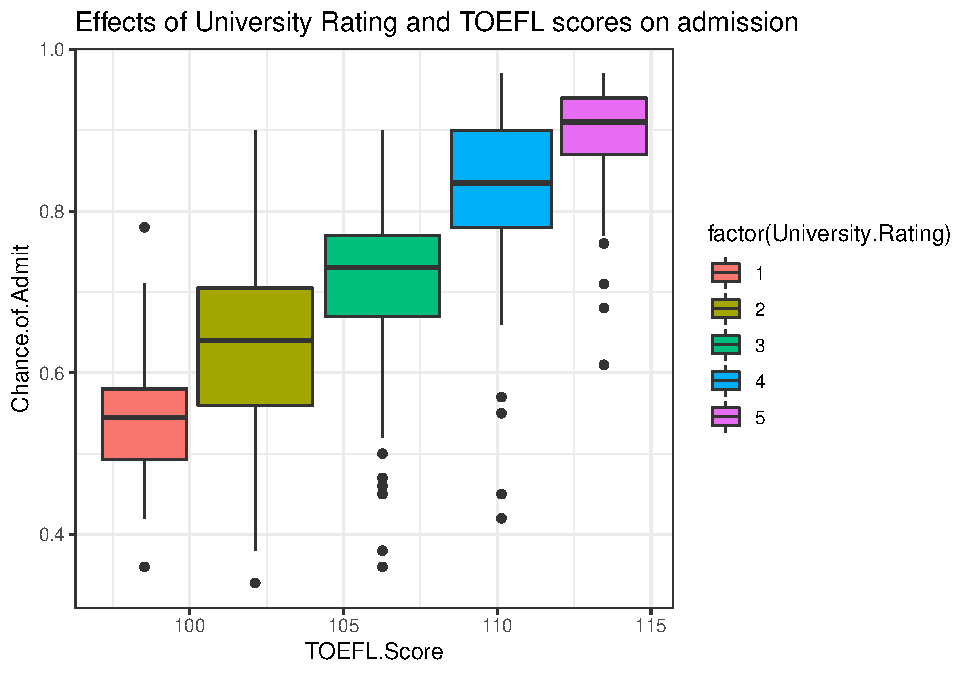
\includegraphics{USGradAdmission_files/figure-latex/unnamed-chunk-6-1.pdf}

\begin{Shaded}
\begin{Highlighting}[]
\NormalTok{adm}\OperatorTok\StringTok{ }
\StringTok{  }\KeywordTok{ggplot}\NormalTok{(}\KeywordTok{aes}\NormalTok{(}\DataTypeTok{x=}\NormalTok{GRE.Score,}
             \DataTypeTok{y=}\NormalTok{Chance.of.Admit, }\DataTypeTok{fill=}\KeywordTok{factor}\NormalTok{(University.Rating))) }\OperatorTok{+}
\StringTok{  }\KeywordTok{geom_boxplot}\NormalTok{() }\OperatorTok{+}\KeywordTok{theme_bw}\NormalTok{()}\OperatorTok{+}
\StringTok{  }\KeywordTok{ggtitle}\NormalTok{(}\StringTok{"Effects of University Rating and GRE scores on admission"}\NormalTok{)}
\end{Highlighting}
\end{Shaded}

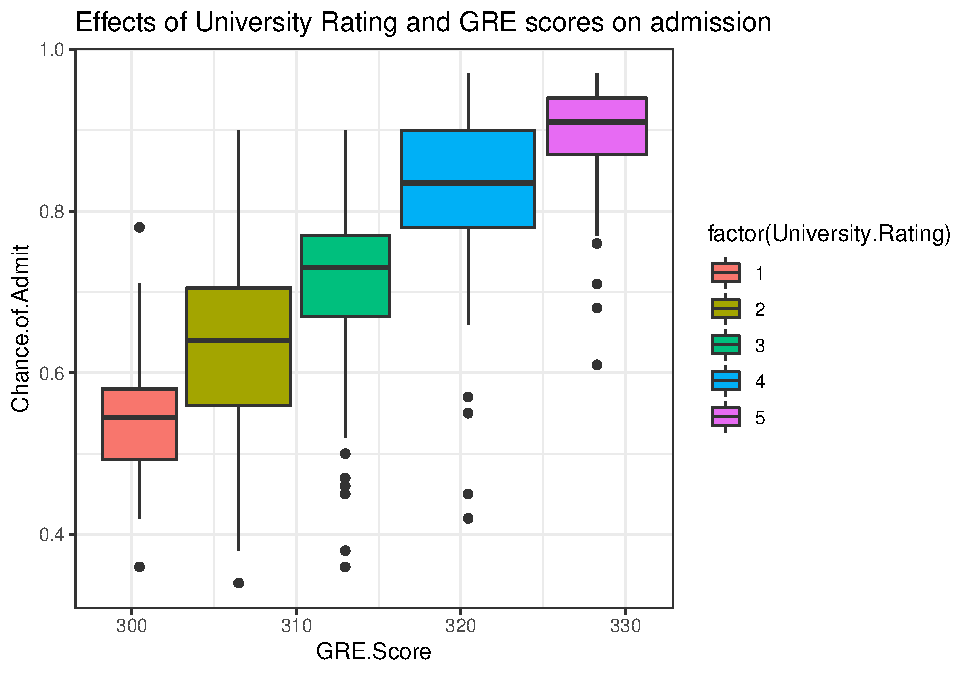
\includegraphics{USGradAdmission_files/figure-latex/unnamed-chunk-6-2.pdf}

\begin{Shaded}
\begin{Highlighting}[]
\NormalTok{adm}\OperatorTok\StringTok{ }
\StringTok{  }\KeywordTok{ggplot}\NormalTok{(}\KeywordTok{aes}\NormalTok{(}\DataTypeTok{x=}\NormalTok{CGPA,}\DataTypeTok{y=}\NormalTok{Chance.of.Admit, }\DataTypeTok{fill=}\KeywordTok{factor}\NormalTok{(University.Rating))) }\OperatorTok{+}
\StringTok{  }\KeywordTok{geom_boxplot}\NormalTok{() }\OperatorTok{+}\KeywordTok{theme_bw}\NormalTok{()}\OperatorTok{+}
\StringTok{  }\KeywordTok{ggtitle}\NormalTok{(}\StringTok{"Effects of University Rating and CGPA scores on admission"}\NormalTok{)}
\end{Highlighting}
\end{Shaded}

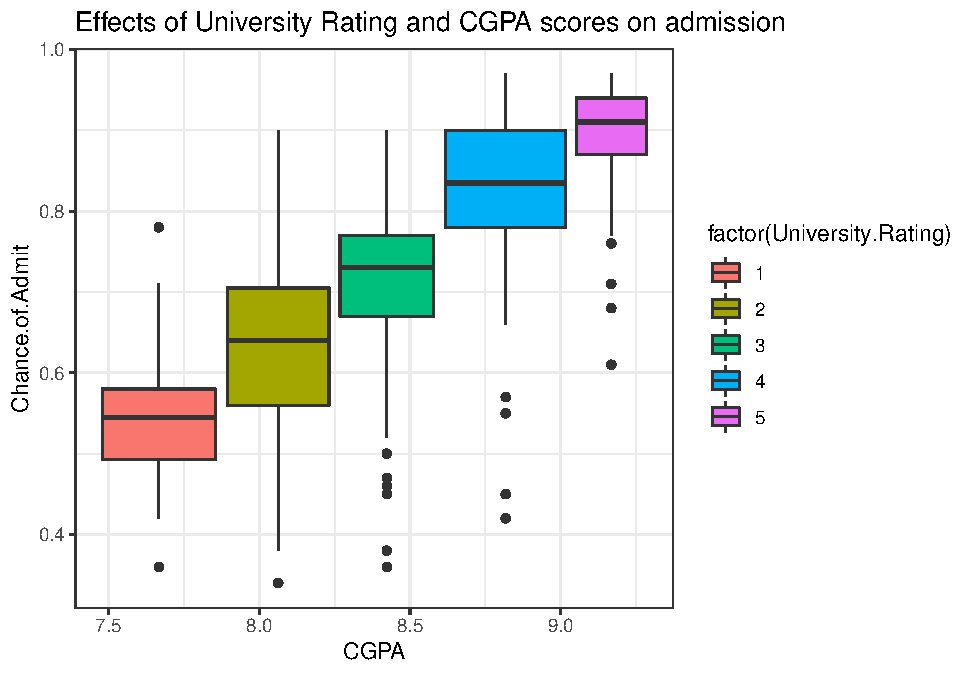
\includegraphics{USGradAdmission_files/figure-latex/unnamed-chunk-6-3.pdf}

\hypertarget{partial-correlation-coefficient}{%
\subsection{Partial correlation
coefficient}\label{partial-correlation-coefficient}}

Beyond the correlation coefficients, the partial correlations reveal the
influence of invidual attribute to our dependent varaible of interest.
Furthermore, partial correlation ensures that the confounding effects of
variables are eliminated. This analysis show that the SOP and
University.Rating had a minor influence when partial correlation values
are considered. Based on these findings SOP, University.Rating will be
cleansed from our datasets before our modeling efforts.

\begin{Shaded}
\begin{Highlighting}[]
\NormalTok{partials=}\KeywordTok{pcor}\NormalTok{(adm_mat) }\CommentTok{# Conducting partial correlation analysis}
\KeywordTok{print}\NormalTok{(}\StringTok{"Partial Correlations for the Dependent Variable: Rent"}\NormalTok{)}
\end{Highlighting}
\end{Shaded}

\begin{verbatim}
## [1] "Partial Correlations for the Dependent Variable: Rent"
\end{verbatim}

\begin{Shaded}
\begin{Highlighting}[]
\NormalTok{Estimates=}\KeywordTok{data.frame}\NormalTok{(partials}\OperatorTok{$}\NormalTok{estimate[,}\DecValTok{7}\OperatorTok{:}\DecValTok{8}\NormalTok{])}
\NormalTok{P.values=}\KeywordTok{data.frame}\NormalTok{(partials}\OperatorTok{$}\NormalTok{p.value[, }\DecValTok{7}\OperatorTok{:}\DecValTok{8}\NormalTok{])}
\CommentTok{# printing the results}
\KeywordTok{kable}\NormalTok{((Estimates), }\DataTypeTok{format =} \StringTok{"markdown"}\NormalTok{, }\DataTypeTok{digits=}\DecValTok{2}\NormalTok{, }
      \DataTypeTok{caption=}\StringTok{"Partial correlations  of the input dataset attributes"}\NormalTok{) }
\end{Highlighting}
\end{Shaded}

\begin{longtable}[]{@{}lrr@{}}
\toprule
& Research & Chance.of.Admit\tabularnewline
\midrule
\endhead
GRE.Score & 0.26 & 0.15\tabularnewline
TOEFL.Score & -0.07 & 0.13\tabularnewline
University.Rating & 0.01 & 0.06\tabularnewline
SOP & 0.08 & -0.03\tabularnewline
LOR & -0.01 & 0.20\tabularnewline
CGPA & -0.05 & 0.44\tabularnewline
Research & 1.00 & 0.15\tabularnewline
Chance.of.Admit & 0.15 & 1.00\tabularnewline
\bottomrule
\end{longtable}

\begin{Shaded}
\begin{Highlighting}[]
\KeywordTok{kable}\NormalTok{((P.values), }\DataTypeTok{format =} \StringTok{"markdown"}\NormalTok{, }\DataTypeTok{digits=}\DecValTok{2}\NormalTok{, }
      \DataTypeTok{caption=}\StringTok{"Probability values  of the input dataset attributes"}\NormalTok{) }
\end{Highlighting}
\end{Shaded}

\begin{longtable}[]{@{}lrr@{}}
\toprule
& Research & Chance.of.Admit\tabularnewline
\midrule
\endhead
GRE.Score & 0.00 & 0.00\tabularnewline
TOEFL.Score & 0.17 & 0.01\tabularnewline
University.Rating & 0.78 & 0.23\tabularnewline
SOP & 0.10 & 0.55\tabularnewline
LOR & 0.87 & 0.00\tabularnewline
CGPA & 0.36 & 0.00\tabularnewline
Research & 0.00 & 0.00\tabularnewline
Chance.of.Admit & 0.00 & 0.00\tabularnewline
\bottomrule
\end{longtable}

\hypertarget{data-preparation-for-modeling}{%
\section{Data Preparation for
Modeling}\label{data-preparation-for-modeling}}

\#\#Data Cleansing Based on the partial correlation coefficient
analysis, the SOP and the University Rating features are removed from
the dataset.

\begin{Shaded}
\begin{Highlighting}[]
\NormalTok{adm}\OperatorTok\NormalTok{dplyr}\OperatorTok{::}\KeywordTok{select}\NormalTok{(}\OperatorTok{-}\NormalTok{SOP, }\OperatorTok{-}\NormalTok{University.Rating)->admfea }\CommentTok{# data cleansed after removing SOP}
\end{Highlighting}
\end{Shaded}

\hypertarget{splitting-data-into-training-and-validation-datasets.}{%
\subsection{Splitting data into training and validation
datasets.}\label{splitting-data-into-training-and-validation-datasets.}}

The data is split into two datasets. One for training and validation.
The training dataset will be used for model development and the
validation dataset will only be used for validation of the model as a
final step. Twenty percent of the cleansed data was chosen as the
validation dataset at random (318) and the rest (82) was saved as the
training dataset. The attributes selected were GRE.Score, TOEFL.Score,
University.Rating, LOR, CGPA and Research

\begin{Shaded}
\begin{Highlighting}[]
\NormalTok{test_indices=}\KeywordTok{createDataPartition}\NormalTok{(admfea}\OperatorTok{$}\NormalTok{Chance.of.Admit, }
                                 \DataTypeTok{times=}\DecValTok{1}\NormalTok{, }
                                 \DataTypeTok{p=}\FloatTok{0.5}\NormalTok{, }\CommentTok{# portion of data split into test}
                                 \DataTypeTok{list=}\NormalTok{F)}
\NormalTok{admfea[}\OperatorTok{-}\NormalTok{test_indices,]->traindf }\CommentTok{# dataset reserved for training}
\NormalTok{admfea[test_indices,]->valdf }\CommentTok{# dataset held for validation}
\end{Highlighting}
\end{Shaded}

\hypertarget{approach-and-model-development}{%
\section{Approach and Model
Development}\label{approach-and-model-development}}

From the data types, boxplots and intial data exploration, it is evident
that this is a regression problem. Accordingly, regression based
modeling solutions will be explored for model development. Initially, a
general linear model will be built using all of the features in the
datasets. Following this a feature reduction step will be performed for
the linear models using a Stepwise regression. A backward and foward
propagated stepwise regression will be performed and the model that
exhibits the lowest AIC score will be selected. The AIC refers to the
Akaike Information Criteria that defines the performance of the model
chosen through a penalization procedure.

\begin{Shaded}
\begin{Highlighting}[]
\CommentTok{# cl=makePSOCKcluster(detectCores())}
\CommentTok{# registerDoParallel(cl)}
\CommentTok{# #Create control function for training with 10 folds}
\CommentTok{# #and keep 3 folds for training. search method is grid.}
\CommentTok{# }
\CommentTok{# control <- trainControl(method='repeatedcv',}
\CommentTok{#                         number=10,}
\CommentTok{#                         repeats=3,}
\CommentTok{#                         search='grid')}
\CommentTok{# }
\CommentTok{# tunegrid <- expand.grid(predFixed = c(1:5), minNode=1:3)}
\CommentTok{# rf_gridsearch <- train(Chance.of.Admit ~ .,}
\CommentTok{#                        data = trainset,}
\CommentTok{#                        method = 'Rborist',}
\CommentTok{#                        metric = c("RMSE"),}
\CommentTok{#                       tuneGrid = tunegrid)}
\CommentTok{# print(rf_gridsearch)}
\CommentTok{# stopCluster(cl)}
\end{Highlighting}
\end{Shaded}

\hypertarget{linear-model}{%
\subsection{Linear Model}\label{linear-model}}

\begin{Shaded}
\begin{Highlighting}[]
\NormalTok{mod.lm=}\KeywordTok{lm}\NormalTok{(Chance.of.Admit}\OperatorTok{~}\NormalTok{., }\DataTypeTok{data=}\NormalTok{traindf)}
\NormalTok{pred.lm=}\KeywordTok{predict}\NormalTok{(mod.lm, }\DataTypeTok{newdata=}\NormalTok{valdf)}
\KeywordTok{RMSE}\NormalTok{(pred.lm, valdf}\OperatorTok{$}\NormalTok{Chance.of.Admit)}
\end{Highlighting}
\end{Shaded}

\begin{verbatim}
## [1] 0.06337683
\end{verbatim}

\begin{Shaded}
\begin{Highlighting}[]
\KeywordTok{stepAIC}\NormalTok{(mod.lm, }\DataTypeTok{direction=}\StringTok{"both"}\NormalTok{)}
\end{Highlighting}
\end{Shaded}

\begin{verbatim}
## Start:  AIC=-1077.91
## Chance.of.Admit ~ GRE.Score + TOEFL.Score + LOR + CGPA + Research
## 
##               Df Sum of Sq     RSS     AIC
## - TOEFL.Score  1   0.00077 0.83303 -1079.7
## <none>                     0.83226 -1077.9
## - GRE.Score    1   0.01578 0.84804 -1076.2
## - Research     1   0.01967 0.85193 -1075.3
## - LOR          1   0.04888 0.88114 -1068.5
## - CGPA         1   0.31951 1.15177 -1015.2
## 
## Step:  AIC=-1079.72
## Chance.of.Admit ~ GRE.Score + LOR + CGPA + Research
## 
##               Df Sum of Sq     RSS     AIC
## <none>                     0.83303 -1079.7
## + TOEFL.Score  1   0.00077 0.83226 -1077.9
## - Research     1   0.01937 0.85240 -1077.2
## - GRE.Score    1   0.02355 0.85658 -1076.2
## - LOR          1   0.04961 0.88264 -1070.2
## - CGPA         1   0.38380 1.21682 -1006.3
\end{verbatim}

\begin{verbatim}
## 
## Call:
## lm(formula = Chance.of.Admit ~ GRE.Score + LOR + CGPA + Research, 
##     data = traindf)
## 
## Coefficients:
## (Intercept)    GRE.Score          LOR         CGPA     Research  
##   -1.213402     0.001827     0.023654     0.146315     0.025734
\end{verbatim}

\begin{Shaded}
\begin{Highlighting}[]
\NormalTok{mod.lm.step=}\KeywordTok{lm}\NormalTok{(Chance.of.Admit}\OperatorTok{~}\NormalTok{GRE.Score}\OperatorTok{+}
\StringTok{                 }\NormalTok{TOEFL.Score}\OperatorTok{+}\NormalTok{LOR}\OperatorTok{+}\NormalTok{CGPA, }\DataTypeTok{data=}\NormalTok{traindf)}
\KeywordTok{summary}\NormalTok{(mod.lm.step)}
\end{Highlighting}
\end{Shaded}

\begin{verbatim}
## 
## Call:
## lm(formula = Chance.of.Admit ~ GRE.Score + TOEFL.Score + LOR + 
##     CGPA, data = traindf)
## 
## Residuals:
##      Min       1Q   Median       3Q      Max 
## -0.23796 -0.01987  0.01154  0.03992  0.14565 
## 
## Coefficients:
##               Estimate Std. Error t value Pr(>|t|)    
## (Intercept) -1.3996427  0.1555292  -8.999  < 2e-16 ***
## GRE.Score    0.0023099  0.0008240   2.803 0.005572 ** 
## TOEFL.Score  0.0004945  0.0015119   0.327 0.743955    
## LOR          0.0252382  0.0069987   3.606 0.000395 ***
## CGPA         0.1449749  0.0168360   8.611 2.48e-15 ***
## ---
## Signif. codes:  0 '***' 0.001 '**' 0.01 '*' 0.05 '.' 0.1 ' ' 1
## 
## Residual standard error: 0.06627 on 194 degrees of freedom
## Multiple R-squared:  0.7925, Adjusted R-squared:  0.7882 
## F-statistic: 185.2 on 4 and 194 DF,  p-value: < 2.2e-16
\end{verbatim}

\hypertarget{machine-learning-models}{%
\subsection{Machine Learning Models}\label{machine-learning-models}}

\begin{Shaded}
\begin{Highlighting}[]
\NormalTok{knitr}\OperatorTok{::}\NormalTok{opts_chunk}\OperatorTok{$}\KeywordTok{set}\NormalTok{(}\DataTypeTok{cache=}\NormalTok{T)}
 
\KeywordTok{set.seed}\NormalTok{(}\DecValTok{1}\NormalTok{)}
 
\NormalTok{cl=}\KeywordTok{makePSOCKcluster}\NormalTok{(}\KeywordTok{detectCores}\NormalTok{()}\OperatorTok{-}\DecValTok{1}\NormalTok{)}
\KeywordTok{registerDoParallel}\NormalTok{(cl)}

\NormalTok{my.con=}\KeywordTok{trainControl}\NormalTok{(}\DataTypeTok{method=}\StringTok{"cv"}\NormalTok{, }\DataTypeTok{number=}\DecValTok{3}\NormalTok{,}
                    \DataTypeTok{savePredictions =} \StringTok{"final"}\NormalTok{, }\DataTypeTok{allowParallel =}\NormalTok{ T)}
\NormalTok{models=}\KeywordTok{caretList}\NormalTok{(Chance.of.Admit}\OperatorTok{~}\NormalTok{., }\DataTypeTok{data=}\NormalTok{traindf,}
\DataTypeTok{trainControl=}\NormalTok{my.con, }
\DataTypeTok{methodList =} \KeywordTok{c}\NormalTok{(}\StringTok{"Rborist"}\NormalTok{,  }
               \StringTok{"knn"}\NormalTok{, }
               \StringTok{"glmnet"}\NormalTok{,}
               \StringTok{"xgbLinear"}\NormalTok{,}
               \StringTok{"brnn"}\NormalTok{, }
               \StringTok{"ridge"}\NormalTok{), }
\DataTypeTok{continue_on_fail =}\NormalTok{ T)}
\end{Highlighting}
\end{Shaded}

\begin{verbatim}
## Warning in trControlCheck(x = trControl, y = target): trControl$savePredictions
## not 'all' or 'final'. Setting to 'final' so we can ensemble the models.
\end{verbatim}

\begin{verbatim}
## Warning in trControlCheck(x = trControl, y = target): indexes not defined in
## trControl. Attempting to set them ourselves, so each model in the ensemble will
## have the same resampling indexes.
\end{verbatim}

\begin{verbatim}
## [12:44:33] WARNING: amalgamation/../src/objective/regression_obj.cu:170: reg:linear is now deprecated in favor of reg:squarederror.
## [12:44:33] WARNING: amalgamation/../src/learner.cc:480: 
## Parameters: { trainControl } might not be used.
## 
##   This may not be accurate due to some parameters are only used in language bindings but
##   passed down to XGBoost core.  Or some parameters are not used but slip through this
##   verification. Please open an issue if you find above cases.
## 
## 
## Number of parameters (weights and biases) to estimate: 7 
## Nguyen-Widrow method
## Scaling factor= 0.7 
## gamma= 6.5184     alpha= 1.228    beta= 10.6021 
## 1 package is needed for this model and is not installed. (elasticnet). Would you like to try to install it now?
\end{verbatim}

\begin{Shaded}
\begin{Highlighting}[]
\NormalTok{models}\OperatorTok{$}\NormalTok{xgbLinear}
\end{Highlighting}
\end{Shaded}

\begin{verbatim}
## eXtreme Gradient Boosting 
## 
## 199 samples
##   5 predictor
## 
## No pre-processing
## Resampling: Bootstrapped (25 reps) 
## Summary of sample sizes: 199, 199, 199, 199, 199, 199, ... 
## Resampling results across tuning parameters:
## 
##   lambda  alpha  nrounds  RMSE        Rsquared   MAE       
##   0e+00   0e+00   50      0.08205874  0.7005220  0.06067428
##   0e+00   0e+00  100      0.08205872  0.7005220  0.06067422
##   0e+00   0e+00  150      0.08205868  0.7005220  0.06067416
##   0e+00   1e-04   50      0.08151685  0.7034346  0.06004102
##   0e+00   1e-04  100      0.08151681  0.7034346  0.06004095
##   0e+00   1e-04  150      0.08151678  0.7034345  0.06004090
##   0e+00   1e-01   50      0.07677988  0.7323696  0.05711481
##   0e+00   1e-01  100      0.07677988  0.7323696  0.05711481
##   0e+00   1e-01  150      0.07677988  0.7323696  0.05711481
##   1e-04   0e+00   50      0.08203076  0.7006150  0.06065748
##   1e-04   0e+00  100      0.08203073  0.7006150  0.06065741
##   1e-04   0e+00  150      0.08203069  0.7006150  0.06065735
##   1e-04   1e-04   50      0.08168928  0.7021681  0.06018655
##   1e-04   1e-04  100      0.08168926  0.7021680  0.06018650
##   1e-04   1e-04  150      0.08168923  0.7021680  0.06018645
##   1e-04   1e-01   50      0.07677987  0.7323933  0.05712004
##   1e-04   1e-01  100      0.07677987  0.7323933  0.05712004
##   1e-04   1e-01  150      0.07677987  0.7323933  0.05712004
##   1e-01   0e+00   50      0.08073932  0.7088634  0.05964312
##   1e-01   0e+00  100      0.08073930  0.7088633  0.05964307
##   1e-01   0e+00  150      0.08073926  0.7088633  0.05964301
##   1e-01   1e-04   50      0.08055568  0.7103941  0.05971346
##   1e-01   1e-04  100      0.08055568  0.7103941  0.05971341
##   1e-01   1e-04  150      0.08055566  0.7103941  0.05971336
##   1e-01   1e-01   50      0.07691574  0.7308336  0.05731010
##   1e-01   1e-01  100      0.07691574  0.7308336  0.05731010
##   1e-01   1e-01  150      0.07691574  0.7308336  0.05731010
## 
## Tuning parameter 'eta' was held constant at a value of 0.3
## RMSE was used to select the optimal model using the smallest value.
## The final values used for the model were nrounds = 50, lambda = 1e-04, alpha
##  = 0.1 and eta = 0.3.
\end{verbatim}

\begin{Shaded}
\begin{Highlighting}[]
\NormalTok{models}\OperatorTok{$}\NormalTok{knn}
\end{Highlighting}
\end{Shaded}

\begin{verbatim}
## k-Nearest Neighbors 
## 
## 199 samples
##   5 predictor
## 
## No pre-processing
## Resampling: Bootstrapped (25 reps) 
## Summary of sample sizes: 199, 199, 199, 199, 199, 199, ... 
## Resampling results across tuning parameters:
## 
##   k  RMSE        Rsquared   MAE       
##   5  0.09306460  0.6055756  0.06961677
##   7  0.09018177  0.6273696  0.06787979
##   9  0.08941066  0.6365068  0.06740945
## 
## RMSE was used to select the optimal model using the smallest value.
## The final value used for the model was k = 9.
\end{verbatim}

\begin{Shaded}
\begin{Highlighting}[]
\NormalTok{models}\OperatorTok{$}\NormalTok{Rborist}
\end{Highlighting}
\end{Shaded}

\begin{verbatim}
## Random Forest 
## 
## 199 samples
##   5 predictor
## 
## No pre-processing
## Resampling: Bootstrapped (25 reps) 
## Summary of sample sizes: 199, 199, 199, 199, 199, 199, ... 
## Resampling results across tuning parameters:
## 
##   predFixed  RMSE        Rsquared   MAE       
##   2          0.07007374  0.7738223  0.05219741
##   3          0.07140460  0.7648293  0.05306859
##   5          0.07411851  0.7471535  0.05481163
## 
## Tuning parameter 'minNode' was held constant at a value of 3
## RMSE was used to select the optimal model using the smallest value.
## The final values used for the model were predFixed = 2 and minNode = 3.
\end{verbatim}

\begin{Shaded}
\begin{Highlighting}[]
\NormalTok{models}\OperatorTok{$}\NormalTok{glmnet}
\end{Highlighting}
\end{Shaded}

\begin{verbatim}
## glmnet 
## 
## 199 samples
##   5 predictor
## 
## No pre-processing
## Resampling: Bootstrapped (25 reps) 
## Summary of sample sizes: 199, 199, 199, 199, 199, 199, ... 
## Resampling results across tuning parameters:
## 
##   alpha  lambda        RMSE        Rsquared   MAE       
##   0.10   0.0002514148  0.06702287  0.7923582  0.04860223
##   0.10   0.0025141476  0.06687991  0.7935777  0.04839192
##   0.10   0.0251414757  0.06810763  0.7930261  0.04933138
##   0.55   0.0002514148  0.06701280  0.7924638  0.04861109
##   0.55   0.0025141476  0.06682233  0.7941896  0.04839073
##   0.55   0.0251414757  0.07051156  0.7943757  0.05291759
##   1.00   0.0002514148  0.06700746  0.7924666  0.04863224
##   1.00   0.0025141476  0.06691587  0.7939357  0.04855497
##   1.00   0.0251414757  0.07423164  0.7888777  0.05742705
## 
## RMSE was used to select the optimal model using the smallest value.
## The final values used for the model were alpha = 0.55 and lambda = 0.002514148.
\end{verbatim}

\begin{Shaded}
\begin{Highlighting}[]
\NormalTok{models}\OperatorTok{$}\NormalTok{brnn}
\end{Highlighting}
\end{Shaded}

\begin{verbatim}
## Bayesian Regularized Neural Networks 
## 
## 199 samples
##   5 predictor
## 
## No pre-processing
## Resampling: Bootstrapped (25 reps) 
## Summary of sample sizes: 199, 199, 199, 199, 199, 199, ... 
## Resampling results across tuning parameters:
## 
##   neurons  RMSE        Rsquared   MAE       
##   1        0.06776434  0.7872853  0.04909314
##   2        0.06860481  0.7821797  0.04978834
##   3        0.07133352  0.7642993  0.05161799
## 
## RMSE was used to select the optimal model using the smallest value.
## The final value used for the model was neurons = 1.
\end{verbatim}

\begin{Shaded}
\begin{Highlighting}[]
\KeywordTok{stopCluster}\NormalTok{(cl)}
\KeywordTok{varImp}\NormalTok{(models}\OperatorTok{$}\NormalTok{Rborist)}
\end{Highlighting}
\end{Shaded}

\begin{verbatim}
## Rborist variable importance
## 
##             Overall
## CGPA         100.00
## GRE.Score     42.11
## TOEFL.Score   26.11
## LOR           14.41
## Research       0.00
\end{verbatim}

\begin{Shaded}
\begin{Highlighting}[]
\KeywordTok{varImp}\NormalTok{(models}\OperatorTok{$}\NormalTok{glmnet)}
\end{Highlighting}
\end{Shaded}

\begin{verbatim}
## glmnet variable importance
## 
##              Overall
## CGPA        100.0000
## Research     17.1930
## LOR          16.2224
## GRE.Score     0.6967
## TOEFL.Score   0.0000
\end{verbatim}

\hypertarget{model-with-reduced-features}{%
\subsection{Model with Reduced
Features}\label{model-with-reduced-features}}

\begin{Shaded}
\begin{Highlighting}[]
\CommentTok{# traindf%>%dplyr::select(-Research, -SOP)->traindf_red}
\CommentTok{# cl=makePSOCKcluster(detectCores()-1)}
\CommentTok{# registerDoParallel(cl)}
\CommentTok{# models=caretList(Chance.of.Admit~., data=traindf_red,}
\CommentTok{# trainControl=my.con, }
\CommentTok{# methodList = c("Rborist",  }
\CommentTok{#                "knn", }
\CommentTok{#                "glmnet",}
\CommentTok{#                "xgbLinear",}
\CommentTok{#                "brnn"), }
\CommentTok{# continue_on_fail = T)}
\CommentTok{# models$xgbLinear}
\CommentTok{# models$knn}
\CommentTok{# models$Rborist}
\CommentTok{# models$glmnet}
\CommentTok{# models$brnn}
\CommentTok{# varImp(models$Rborist)}
\CommentTok{# varImp(models$glmnet)}
\end{Highlighting}
\end{Shaded}

\hypertarget{feature-reduction}{%
\subsection{Feature Reduction}\label{feature-reduction}}

\begin{Shaded}
\begin{Highlighting}[]
\KeywordTok{set.seed}\NormalTok{(}\DecValTok{1}\NormalTok{)}
\NormalTok{cl=}\KeywordTok{makePSOCKcluster}\NormalTok{(}\KeywordTok{detectCores}\NormalTok{()}\OperatorTok{-}\DecValTok{1}\NormalTok{)}
\KeywordTok{registerDoParallel}\NormalTok{(cl)}
 
\NormalTok{ctrl=}\KeywordTok{rfeControl}\NormalTok{(}\DataTypeTok{functions =}\NormalTok{ rfFuncs,}
           \DataTypeTok{method =} \StringTok{"cv"}\NormalTok{,}
           \DataTypeTok{number =} \DecValTok{2}\NormalTok{,}
           \DataTypeTok{verbose =}\NormalTok{ F)}
\NormalTok{subsets=}\KeywordTok{c}\NormalTok{(}\DecValTok{1}\OperatorTok{:}\DecValTok{6}\NormalTok{)}
\NormalTok{lmProfile=}\KeywordTok{rfe}\NormalTok{(traindf[,}\OperatorTok{-}\DecValTok{6}\NormalTok{], traindf[,}\DecValTok{6}\NormalTok{], }\DataTypeTok{sizes=}\NormalTok{subsets, }\DataTypeTok{rfeControl=}\NormalTok{ctrl)}
\NormalTok{lmProfile}
\end{Highlighting}
\end{Shaded}

\begin{verbatim}
## 
## Recursive feature selection
## 
## Outer resampling method: Cross-Validated (2 fold) 
## 
## Resampling performance over subset size:
## 
##  Variables    RMSE Rsquared     MAE    RMSESD RsquaredSD    MAESD Selected
##          1 0.07691   0.7143 0.05767 0.0076163    0.05154 0.005530         
##          2 0.07275   0.7463 0.05572 0.0036125    0.02404 0.005764         
##          3 0.07454   0.7453 0.05623 0.0006496    0.01353 0.003492         
##          4 0.07306   0.7545 0.05469 0.0026195    0.01914 0.002431         
##          5 0.07077   0.7762 0.05266 0.0018916    0.02764 0.004516        *
## 
## The top 5 variables (out of 5):
##    CGPA, GRE.Score, LOR, Research, TOEFL.Score
\end{verbatim}

\begin{Shaded}
\begin{Highlighting}[]
\KeywordTok{plot}\NormalTok{(lmProfile)}
\end{Highlighting}
\end{Shaded}

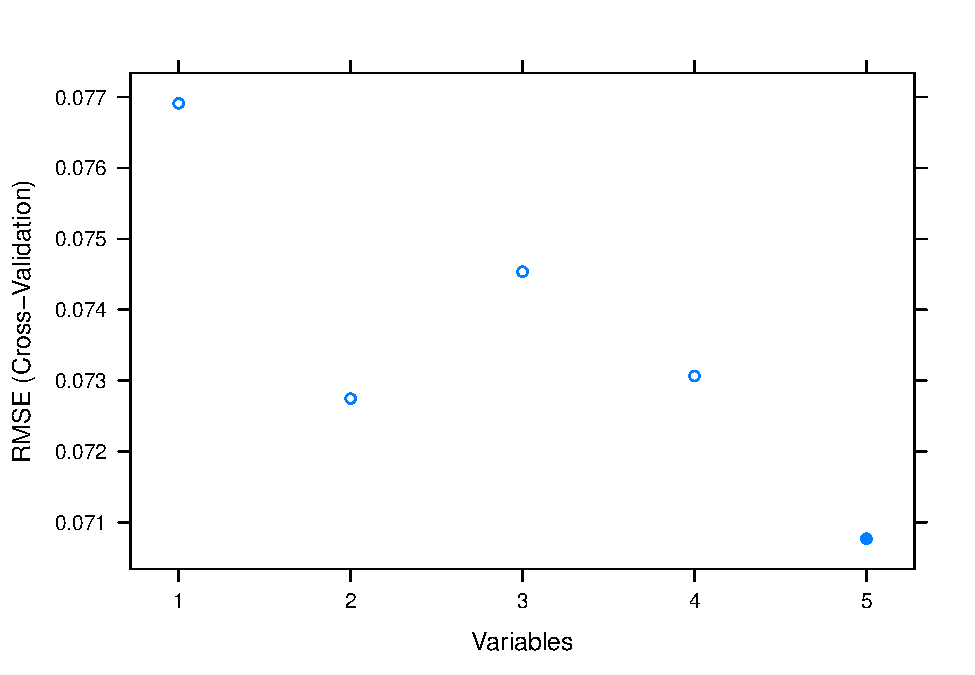
\includegraphics{USGradAdmission_files/figure-latex/unnamed-chunk-14-1.pdf}

\begin{Shaded}
\begin{Highlighting}[]
\NormalTok{ cl=}\KeywordTok{makePSOCKcluster}\NormalTok{(}\KeywordTok{detectCores}\NormalTok{()}\OperatorTok{-}\DecValTok{1}\NormalTok{)}
 \KeywordTok{registerDoParallel}\NormalTok{(cl)}
\NormalTok{ resamples<-}\KeywordTok{resamples}\NormalTok{(models)}
 \KeywordTok{dotplot}\NormalTok{(resamples, }\DataTypeTok{metric=}\StringTok{"RMSE"}\NormalTok{)}
\end{Highlighting}
\end{Shaded}

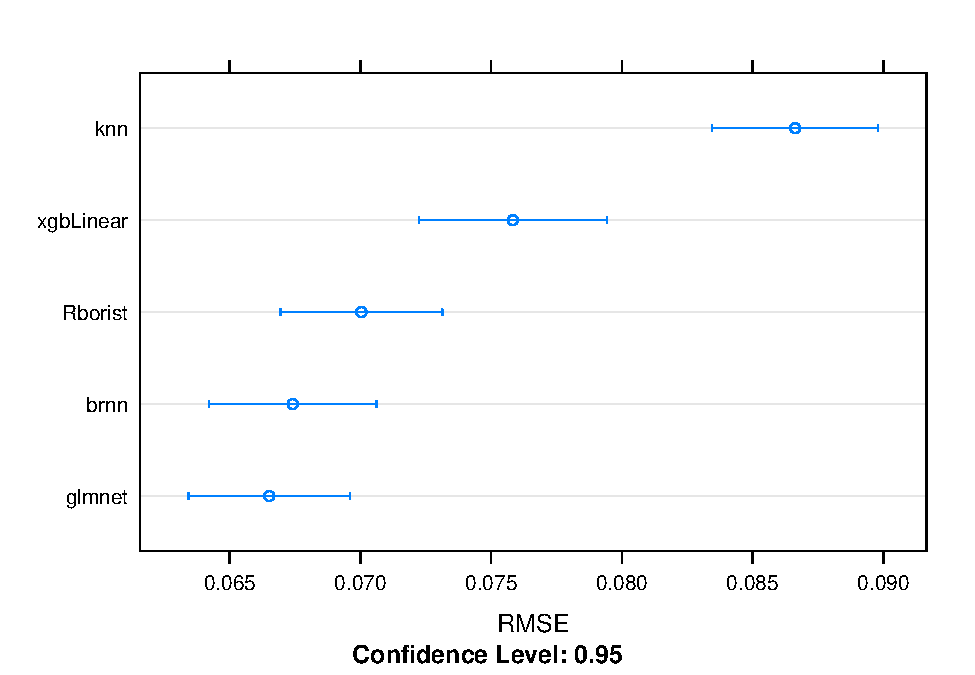
\includegraphics{USGradAdmission_files/figure-latex/unnamed-chunk-15-1.pdf}
\# Results

\begin{Shaded}
\begin{Highlighting}[]
\NormalTok{cl=}\KeywordTok{makePSOCKcluster}\NormalTok{(}\KeywordTok{detectCores}\NormalTok{())}
\KeywordTok{registerDoParallel}\NormalTok{(cl)}
\NormalTok{ens=}\KeywordTok{caretEnsemble}\NormalTok{(models, }\DataTypeTok{metric=}\StringTok{"RMSE"}\NormalTok{, }\DataTypeTok{trControl=}\NormalTok{my.con)}
\KeywordTok{summary}\NormalTok{(ens)}
\end{Highlighting}
\end{Shaded}

\begin{verbatim}
## The following models were ensembled: Rborist, knn, glmnet, xgbLinear, brnn 
## They were weighted: 
## -0.0257 0.1918 0.0711 1.3128 -0.0134 -0.5298
## The resulting RMSE is: 0.0665
## The fit for each individual model on the RMSE is: 
##     method       RMSE      RMSESD
##    Rborist 0.07003540 0.007494216
##        knn 0.08663003 0.007687303
##     glmnet 0.06650807 0.007488198
##  xgbLinear 0.07583018 0.008713204
##       brnn 0.06740915 0.007771737
\end{verbatim}

\begin{Shaded}
\begin{Highlighting}[]
\KeywordTok{plot}\NormalTok{(ens)}
\end{Highlighting}
\end{Shaded}

\begin{verbatim}
## Warning: Duplicated aesthetics after name standardisation: size
\end{verbatim}

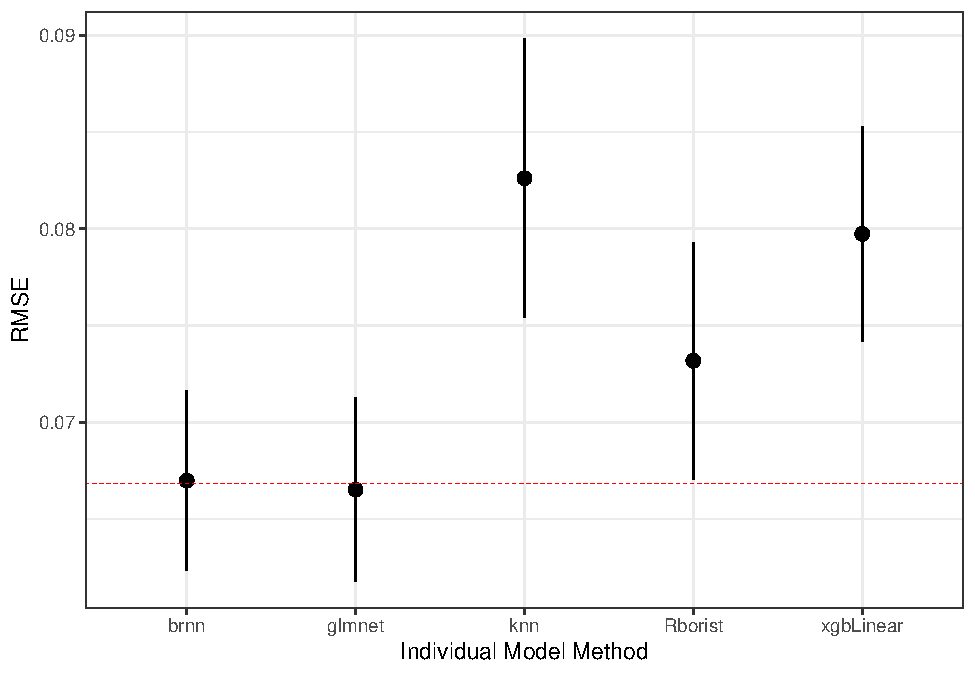
\includegraphics{USGradAdmission_files/figure-latex/unnamed-chunk-16-1.pdf}

\#Validation

In this step, the model are evaluated for their performance. The models
are used to predict the admission probabilities of the students with the
validation dataset which was reserved from participating in the model
developent process. The actual values of the admission rates were
compared to the predicted values from various models. Both RMSE an the
R2 values were evaluated.

\begin{Shaded}
\begin{Highlighting}[]
\CommentTok{#Prediction from Linear model }
\NormalTok{pred.lm.step=}\KeywordTok{predict}\NormalTok{(mod.lm.step, }\DataTypeTok{newdata =}\NormalTok{ valdf) }

\CommentTok{#Predicted from Rborist }

\NormalTok{ predicted.Rborist=}\KeywordTok{predict}\NormalTok{(models}\OperatorTok{$}\NormalTok{Rborist, }\DataTypeTok{newdata=}\NormalTok{valdf)}
 
\CommentTok{#Prediction from Ensemble of the models}
\NormalTok{ predicted.ens=}\KeywordTok{predict}\NormalTok{(ens, }\DataTypeTok{newdata=}\NormalTok{valdf)}
\end{Highlighting}
\end{Shaded}

\begin{verbatim}
## [12:44:42] WARNING: amalgamation/../src/objective/regression_obj.cu:170: reg:linear is now deprecated in favor of reg:squarederror.
\end{verbatim}

\begin{Shaded}
\begin{Highlighting}[]
 \KeywordTok{data.frame}\NormalTok{(}\DataTypeTok{Rborist=}\KeywordTok{RMSE}\NormalTok{(predicted.Rborist, valdf}\OperatorTok{$}\NormalTok{Chance.of.Admit), }
            \DataTypeTok{Ensemble=}\KeywordTok{RMSE}\NormalTok{(predicted.ens, valdf}\OperatorTok{$}\NormalTok{Chance.of.Admit),}
            \DataTypeTok{Linear=}\KeywordTok{RMSE}\NormalTok{(pred.lm.step, valdf}\OperatorTok{$}\NormalTok{Chance.of.Admit))}
\end{Highlighting}
\end{Shaded}

\begin{verbatim}
##      Rborist   Ensemble     Linear
## 1 0.06975151 0.05834425 0.06418429
\end{verbatim}

\begin{Shaded}
\begin{Highlighting}[]
 \KeywordTok{data.frame}\NormalTok{(}\DataTypeTok{Rborist=}\KeywordTok{cor}\NormalTok{(predicted.Rborist, valdf}\OperatorTok{$}\NormalTok{Chance.of.Admit), }
            \DataTypeTok{Ensemble=}\KeywordTok{cor}\NormalTok{(predicted.ens, valdf}\OperatorTok{$}\NormalTok{Chance.of.Admit),}
            \DataTypeTok{Linear=}\KeywordTok{cor}\NormalTok{(pred.lm.step, valdf}\OperatorTok{$}\NormalTok{Chance.of.Admit))}
\end{Highlighting}
\end{Shaded}

\begin{verbatim}
##     Rborist  Ensemble    Linear
## 1 0.8720163 0.9116409 0.8940309
\end{verbatim}

\hypertarget{conclusion}{%
\section{Conclusion}\label{conclusion}}

Comparison was made between a linear regression model and a ensemble
technique with machine learning algorithms for their abilities to
predict the admission probability of applicants to US graduate schools.
The applicant characteristics such as GRE.Score, TOEFL.Score, CGPA, LOR
and SOP were positively correlated with the admission probabilities.
Both linear regression and an ensemble of maching learning algorithms
both predicted the outcomes with great accuracy (RME =0.065 and R2 of
0.88). For this given problem, either of the approaches will work.
Nevertheless, owing to the simplicy of linear model, for practical
purposes, the linear model approach is favored.





\newpage
\singlespacing 
\end{document}